
%(BEGIN_QUESTION)
% Copyright 2010, Tony R. Kuphaldt, released under the Creative Commons Attribution License (v 1.0)
% This means you may do almost anything with this work of mine, so long as you give me proper credit

Suppose this valve control system has a problem.  The control valve (LV-104) does not move to the full-open position as it should when the solenoid is de-energized, although it will move when the 4-20 mA current signal to the I/P transducer is varied while the solenoid is energized:

$$\includegraphics[width=15.5cm]{i04692x01.eps}$$

\vskip 10pt

Identify the likelihood of each specified fault for this circuit.  Consider each fault one at a time (i.e. no coincidental faults), determining whether or not each fault could independently account for {\it all} measurements and symptoms in this circuit.

% No blank lines allowed between lines of an \halign structure!
% I use comments (%) instead, so that TeX doesn't choke.

$$\vbox{\offinterlineskip
\halign{\strut
\vrule \quad\hfil # \ \hfil & 
\vrule \quad\hfil # \ \hfil & 
\vrule \quad\hfil # \ \hfil \vrule \cr
\noalign{\hrule}
%
% First row
{\bf Fault} & {\bf Possible} & {\bf Impossible} \cr
%
\noalign{\hrule}
%
% Another row
Manual valve in ``bypass'' position &  &  \cr
%
\noalign{\hrule}
%
% Another row
Solenoid coil failed open &  &  \cr
%
\noalign{\hrule}
%
% Another row
Solenoid coil failed shorted &  &  \cr
%
\noalign{\hrule}
%
% Another row
Solenoid valve (UY-104) spool stuck &  &  \cr
%
\noalign{\hrule}
%
% Another row
Solenoid valve (UY-104) vent plugged &  &  \cr
%
\noalign{\hrule}
%
% Another row
Air supply to LY-104 failed &  &  \cr
%
\noalign{\hrule}
%
% Another row
4-20 mA signal wiring to LY-104 failed open &  &  \cr
%
\noalign{\hrule}
%
% Another row
4-20 mA signal wiring to LY-104 failed shorted &  &  \cr
%
\noalign{\hrule}
%
% Another row
Control valve (LV-104) stuck &  &  \cr
%
\noalign{\hrule}
} % End of \halign 
}$$ % End of \vbox

\underbar{file i04692}
%(END_QUESTION)





%(BEGIN_ANSWER)

% No blank lines allowed between lines of an \halign structure!
% I use comments (%) instead, so that TeX doesn't choke.

$$\vbox{\offinterlineskip
\halign{\strut
\vrule \quad\hfil # \ \hfil & 
\vrule \quad\hfil # \ \hfil & 
\vrule \quad\hfil # \ \hfil \vrule \cr
\noalign{\hrule}
%
% First row
{\bf Fault} & {\bf Possible} & {\bf Impossible} \cr
%
\noalign{\hrule}
%
% Another row
Manual valve in ``bypass'' position & $\surd$ &  \cr
%
\noalign{\hrule}
%
% Another row
Solenoid coil failed open &  & $\surd$ \cr
%
\noalign{\hrule}
%
% Another row
Solenoid coil failed shorted &  & $\surd$ \cr
%
\noalign{\hrule}
%
% Another row
Solenoid valve (UY-104) spool stuck & $\surd$ &  \cr
%
\noalign{\hrule}
%
% Another row
Solenoid valve (UY-104) vent plugged & $\surd$ &  \cr
%
\noalign{\hrule}
%
% Another row
Air supply to LY-104 failed &  & $\surd$ \cr
%
\noalign{\hrule}
%
% Another row
4-20 mA signal wiring to LY-104 failed open &  & $\surd$ \cr
%
\noalign{\hrule}
%
% Another row
4-20 mA signal wiring to LY-104 failed shorted &  & $\surd$ \cr
%
\noalign{\hrule}
%
% Another row
Control valve (LV-104) stuck &  & $\surd$ \cr
%
\noalign{\hrule}
} % End of \halign 
}$$ % End of \vbox

%(END_ANSWER)





%(BEGIN_NOTES)

\vskip 20pt \vbox{\hrule \hbox{\strut \vrule{} {\bf Virtual Trip-testing} \vrule} \hrule}

This question is a good candidate for a ``Virtual Trip-testing'' exercise.  Presenting the diagram to students, you pose an assignment whereby students must figure out how to test some component of this system to check that it will operate as intended to shut down the system in an abnormal (trip) condition, with some realistic limitation (e.g. power cannot be shut off to the load).  Students then propose various methods for executing the test.  Your job is to determine whether or not their proposed tests will achieve the desired result(s).

During and after the exercise, it is good to ask students follow-up questions such as:

\begin{itemize}
\item{} Where might our planned test strategy go wrong?  In other words, what thing(s) might happen to foil our test, either to invalidate the results or to not honor the stated limitation(s)?
\item{} Suppose the limitation were different.  How would this affect our ability to carry out the test?
\item{} Is the last test strategy best one we could execute?
\end{itemize}



%INDEX% Final Control Elements, valve: fail-safe solenoids

%(END_NOTES)


